\documentclass[aspectratio=169]{../latex_main/tntbeamer}  % you can pass all options of the beamer class, e.g., 'handout' or 'aspectratio=43'
\usepackage{dsfont}
\usepackage{bm}
\usepackage[english]{babel}
\usepackage[T1]{fontenc}
%\usepackage[utf8]{inputenc}
\usepackage{graphicx}
\graphicspath{ {./figures/} }
\usepackage{algorithm}
\usepackage[ruled,vlined,algo2e,linesnumbered]{algorithm2e}
\usepackage{hyperref}
\usepackage{booktabs}
\usepackage{mathtools}

\usepackage{amsmath,amssymb}

\DeclareMathOperator*{\argmax}{arg\,max}
\DeclareMathOperator*{\argmin}{arg\,min}

\usepackage{amsbsy}
\newcommand{\vect}[1]{\bm{#1}}
%\newcommand{\vect}[1]{\boldsymbol{#1}}

\usepackage{pgfplots}
\pgfplotsset{compat=1.16}
\usepackage{tikz}
\usetikzlibrary{trees} 
\usetikzlibrary{shapes.geometric}
\usetikzlibrary{positioning,shapes,shadows,arrows,calc,mindmap}
\usetikzlibrary{positioning,fadings,through}
\usetikzlibrary{decorations.pathreplacing}
\usetikzlibrary{intersections}
\pgfdeclarelayer{background}
\pgfdeclarelayer{foreground}
\pgfsetlayers{background,main,foreground}
\tikzstyle{activity}=[rectangle, draw=black, rounded corners, text centered, text width=8em]
\tikzstyle{data}=[rectangle, draw=black, text centered, text width=8em]
\tikzstyle{myarrow}=[->, thick, draw=black]

% Define the layers to draw the diagram
\pgfdeclarelayer{background}
\pgfdeclarelayer{foreground}
\pgfsetlayers{background,main,foreground}

% Requires XeLaTeX or LuaLaTeX
%\usepackage{unicode-math}

\usepackage{fontspec}
%\setsansfont{Arial}
\setsansfont{RotisSansSerifStd}[ 
Path=../latex_main/fonts/,
Extension = .otf,
UprightFont = *-Regular,  % or *-Light
BoldFont = *-ExtraBold,  % or *-Bold
ItalicFont = *-Italic
]
\setmonofont{Cascadia Mono}[
Scale=0.8
]

\renewcommand{\ttdefault}{Cascadia Mono}

% scale factor adapted; mathrm font added (Benjamin Spitschan @TNT, 2021-06-01)
%\setmathfont[Scale=1.05]{Libertinus Math}
%\setmathrm[Scale=1.05]{Libertinus Math}

% other available math fonts are (not exhaustive)
% Latin Modern Math
% XITS Math
% Libertinus Math
% Asana Math
% Fira Math
% TeX Gyre Pagella Math
% TeX Gyre Bonum Math
% TeX Gyre Schola Math
% TeX Gyre Termes Math

% Literature References
\newcommand{\lit}[2]{\href{#2}{\footnotesize\color{black!60}[#1]}}

%%% Beamer Customization
%----------------------------------------------------------------------
% (Don't) Show sections in frame header. Options: 'sections', 'sections light', empty
\setbeamertemplate{headline}{empty}

% Add header logo for normal frames
\setheaderimage{
	% 
\includegraphics[height=\logoheight]{figures/TNT_darkv4.pdf}
	
\includegraphics[height=\logoheight]{../latex_main/figures/Leibniz-AI-Academy_Logo}
	% 
\includegraphics[height=\logoheight]{figures/logo_tntluh.pdf}
}

% Header logo for title page
\settitleheaderimage{
	% 
\includegraphics[height=\logoheight]{figures/TNT_darkv4.pdf}
	
\includegraphics[height=\logoheight]{../latex_main/figures/Leibniz-AI-Academy_Logo}
	% 
\includegraphics[height=\logoheight]{figures/logo_tntluh.pdf}
}

% Title page: tntdefault 
\setbeamertemplate{title page}[tntdefault]  % or luhstyle
% Add optional title image here
%\addtitlepageimagedefault{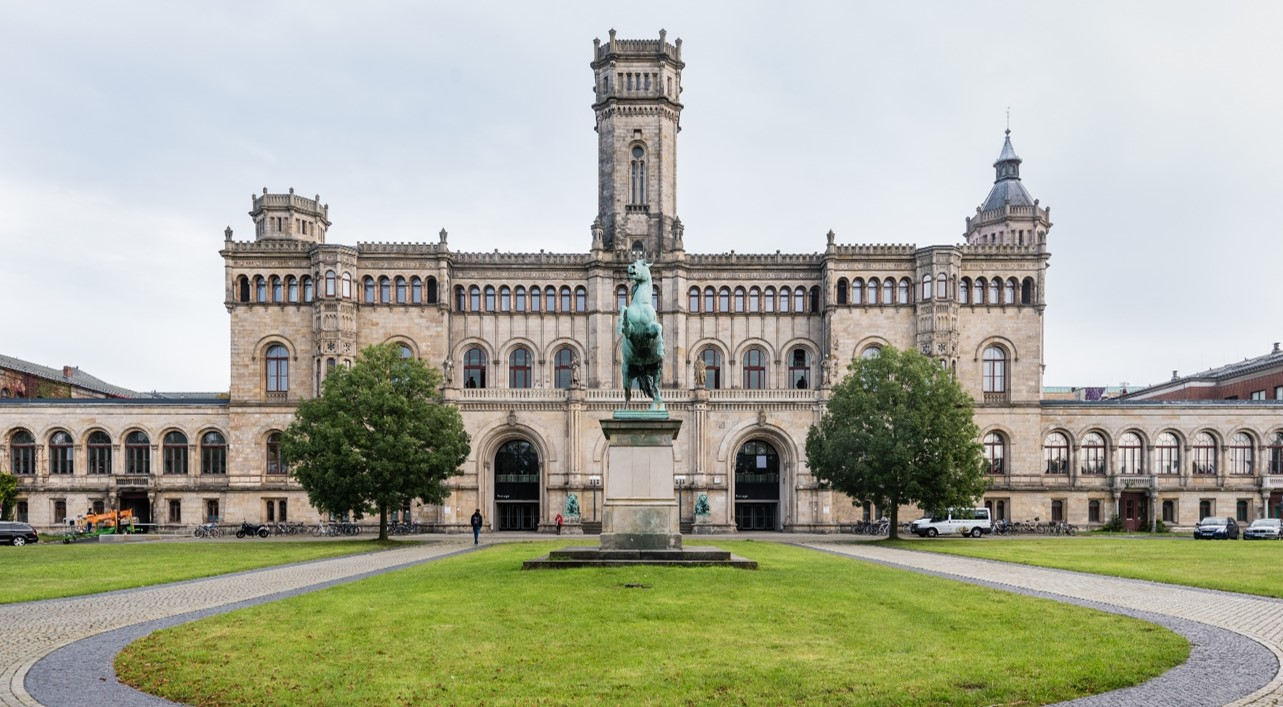
\includegraphics[width=0.65\textwidth]{figures/luh_default_presentation_title_image.jpg}}

% Title page: luhstyle
% \setbeamertemplate{title page}[luhstyle]
% % Add optional title image here
% \addtitlepageimage{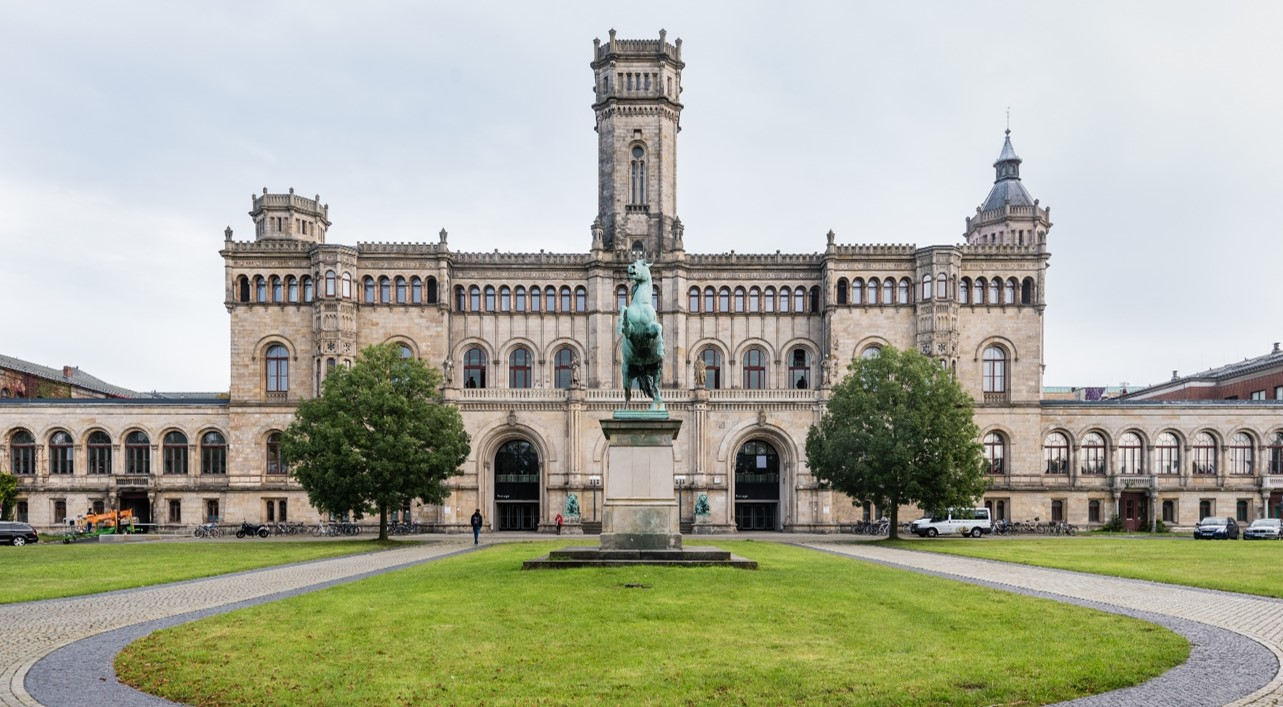
\includegraphics[width=0.75\textwidth]{figures/luh_default_presentation_title_image.jpg}}

\author[Abedjan \& Lindauer]{Ziawasch Abedjan \& \underline{Marius Lindauer}\\[1em]
	%
\includegraphics[height=\logoheight]{../latex_main/figures/luh_logo_rgb_0_80_155.pdf}\qquad
	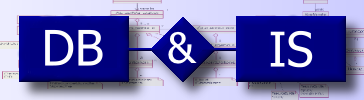
\includegraphics[height=\logoheight]{../latex_main/figures/DBIS_Kurzlogo.png}\qquad
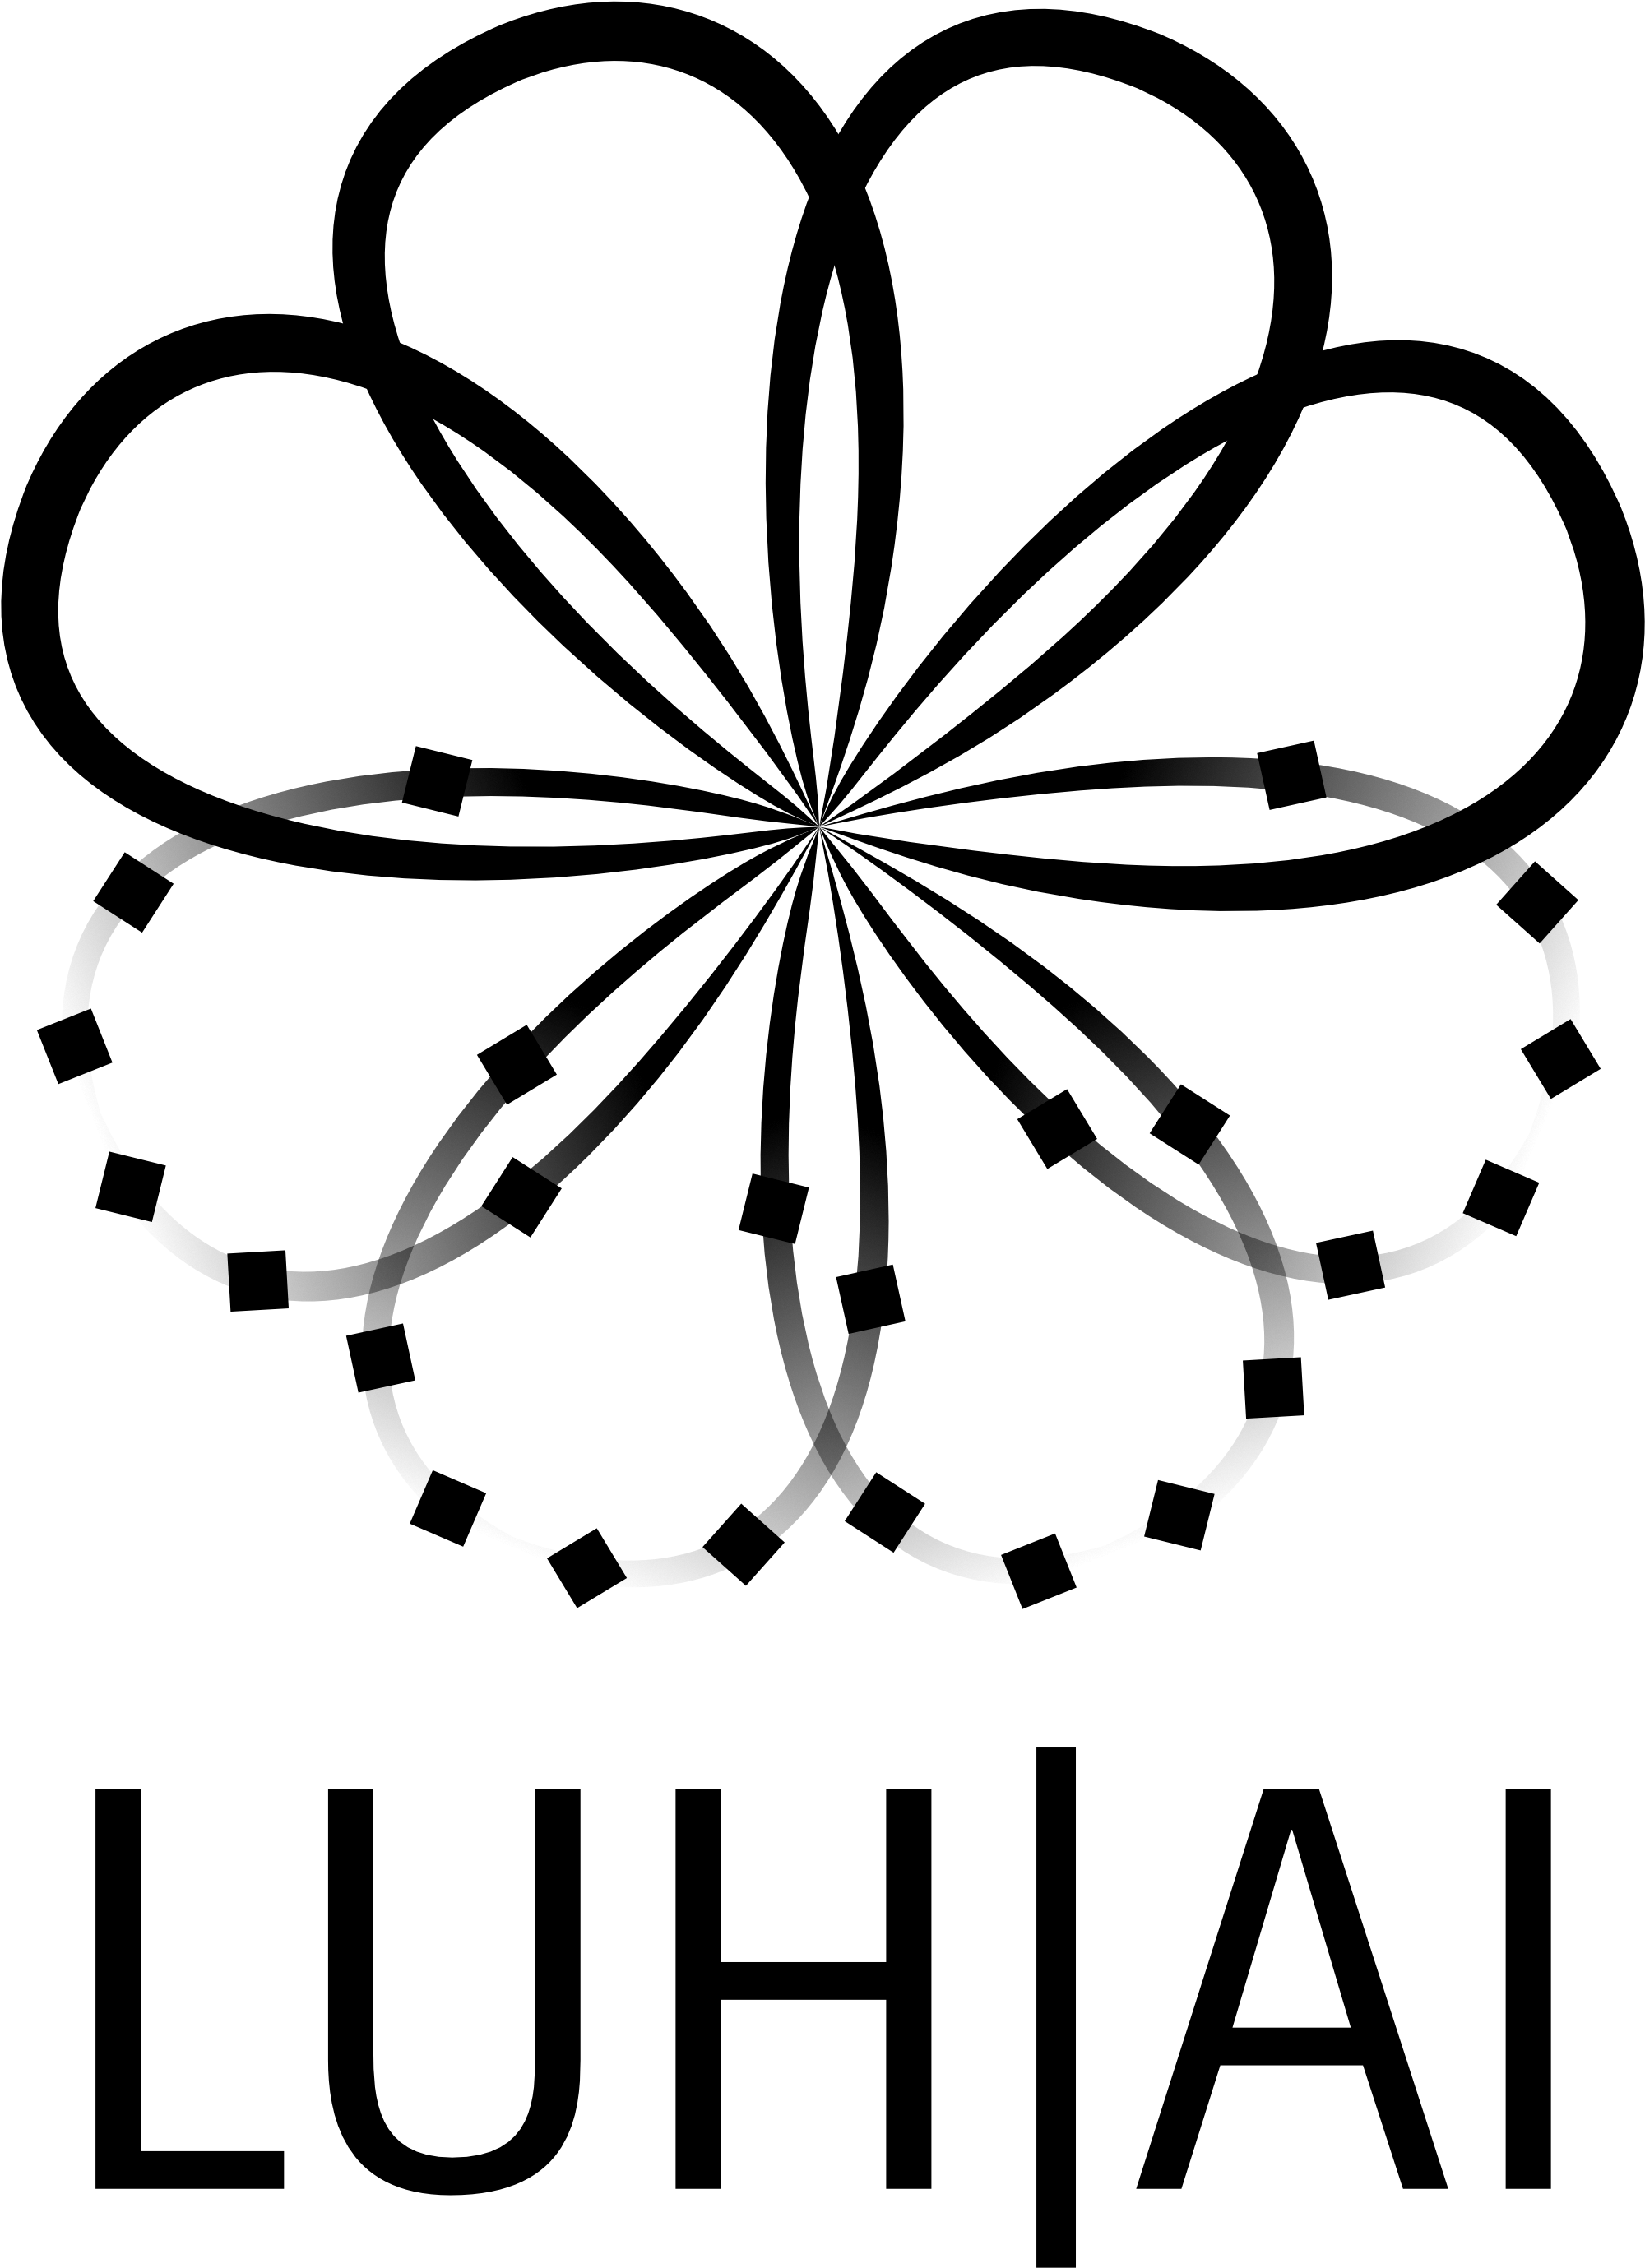
\includegraphics[height=\logoheight]{../latex_main/figures/logo_short_highres_black}\qquad

\includegraphics[height=\logoheight]{../latex_main/figures/Leibniz-AI-Academy_Logo}\qquad
%
\includegraphics[height=\logoheight]{../latex_main/figures/L3S.jpg}	
}
\date{\hspace{0.5em} {
\includegraphics[height=1.5em]{../latex_main/figures/Cc-by-nc-sa_icon.svg.png}}; extension of \href{https://ds100.org/fa21/}{[DS100]}
}


%%% Custom Packages
%----------------------------------------------------------------------
% Create dummy content
\usepackage{blindtext}

% Adds a frame with the current page layout. Just call \layout inside of a frame.
\usepackage{layout}


%%% Macros
%\renewcommand{\vec}[1]{\mathbf{#1}}
% \usepackage{bm}
%\let\vecb\bm

\title[Data Property: Temporality \& Faithfulness]{DS: Data Cleaning}
\subtitle{Data Property: Temporality \& Faithfulness}

\graphicspath{ {./figure/} }
%\institute{}


\begin{document}
	
	\maketitle
 
\begin{frame}[c]{Key Data Properties to Consider in EDA}
    \begin{itemize}
        \item {Structure} -- the “shape” of a data file.
        \item {Granularity} -- how fine/coarse is each datum.
        \item {Scope} -- how (in)complete is the data.
        \item \textbf{Temporality} -- how is the data situated in time.
        \item {Faithfulness} --how well does the data capture “reality”.
    \end{itemize}
\end{frame}


% Slide 34 - Temporality
\begin{frame}[c]{Temporality}

    \begin{itemize}
        \item Data changes – when was the data collected?
        \item What is the meaning of the time and date fields?
        \begin{itemize}
            \item When did the “event” happen?
            \item When the data was collected or was entered into the system?
        \end{itemize}
        \pause
        \item Time depends on where! (Time zones \& daylight savings)
        \begin{itemize}
            \item Learn to use datetime python library
            \item Multiple string representation (depends on region): 07/08/09?
        \end{itemize}
        \pause
        \item Are there hidden null values?
        \begin{itemize}
            \item January 1st 1970, January 1st 1900
        \end{itemize}
        \pause
        \item Is there periodicity? 
        \begin{itemize}
            \item For example Diurnal patterns because most animals are more active at daylight and sleep at night
        \end{itemize}
    \end{itemize}
    
\end{frame}

\begin{frame}{Importance of Data Temporality}

\begin{itemize}
    \item {Tracks Changes Over Time}
    \begin{itemize}
        \item Enables trend analysis, seasonal patterns, and forecasting.
    \end{itemize}
\pause
    \item {Supports Causal Analysis and Predictions}
    \begin{itemize}
        \item Allows for understanding cause-effect relationships and predicting outcomes.
    \end{itemize}
\pause
    \item {Facilitates Time-Based Aggregation and Resampling}
    \begin{itemize}
        \item Allows for appropriate data summarization at different time intervals.
    \end{itemize}
\pause
    \item {Improves Forecasting and Planning}
    \begin{itemize}
        \item Temporal data is essential for accurate predictions in various domains.
    \end{itemize}
\pause
    \item {Supports Seasonal and Cyclical Pattern Identification}
    \begin{itemize}
        \item Crucial for identifying recurring trends (e.g., seasonal sales).
    \end{itemize}
\pause
    \item {Helps Identify Data Recency and Relevance}
    \begin{itemize}
        \item Ensures that data is current and relevant to the analysis context.
    \end{itemize}
\end{itemize}

\end{frame}

\begin{frame}[c]{Key Data Properties to Consider in EDA}
    \begin{itemize}
        \item {Structure} -- the “shape” of a data file.
        \item {Granularity} -- how fine/coarse is each datum.
        \item {Scope} -- how (in)complete is the data.
        \item {Temporality} -- how is the data situated in time.
        \item \textbf{Faithfulness} --how well does the data capture “reality”.
    \end{itemize}
\end{frame}

% Slide 36 - Faithfulness
\begin{frame}[c]{Faithfulness: Trusting the Data}
    \begin{itemize}
        \item Does my data contain unrealistic or “incorrect” values?
        \begin{itemize}
            \item Dates in the future for events in the past, locations that don’t exist
            \item Negative counts, large outliers
            \item Misspellings of names
        \end{itemize}
        \item Does my data violate obvious dependencies?
        \begin{itemize}
            \item E.g., age and birthday don’t match
        \end{itemize}
        \item Was the data entered by hand?
        \begin{itemize}
            \item Spelling errors, fields shifted …
            \item Did the form require fields or provide default values?
        \end{itemize}
        \item Are there obvious signs of data falsification:
        \begin{itemize}
            \item Repeated names, fake looking email addresses, repeated use of uncommon names.
        \end{itemize}
    \end{itemize}
\end{frame}

% Slide 37 - Information Quality
\begin{frame}[c]{Zooming into Information Quality}

    \centering
    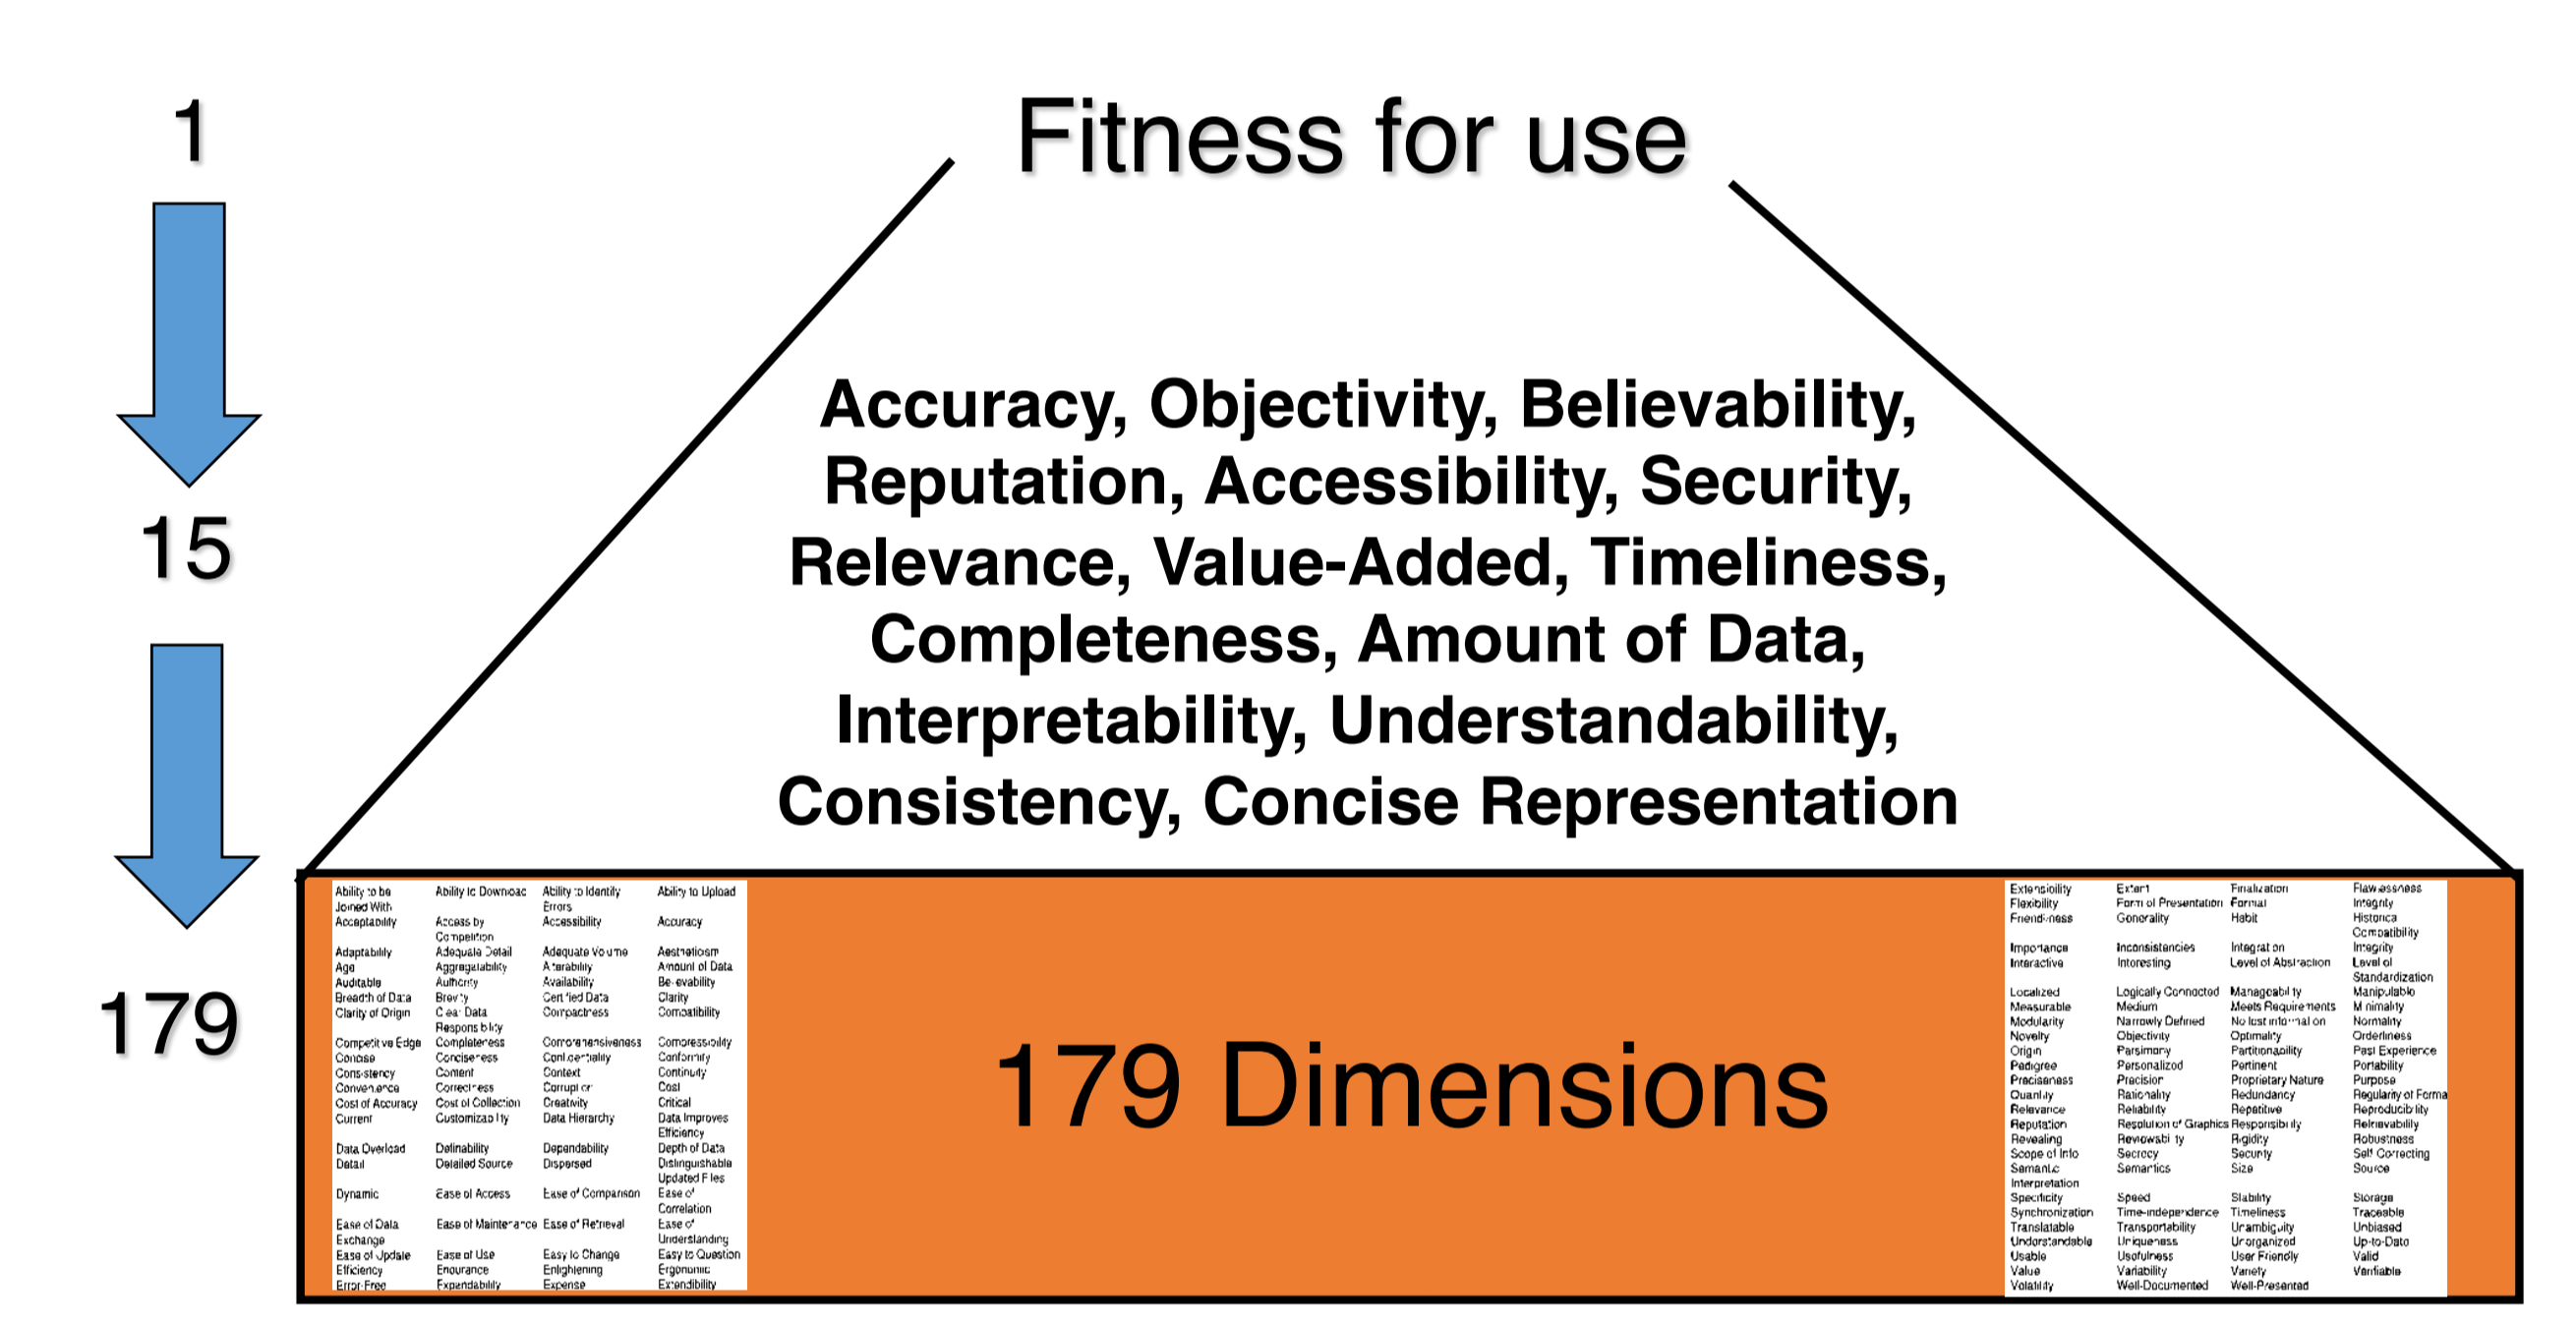
\includegraphics[width=0.8\textwidth]{figure/bild12_information_quality.png}

\end{frame}

% Slide 38 - Data Quality Problems
\begin{frame}[c]{Common Data Quality Problems}
    \centering
    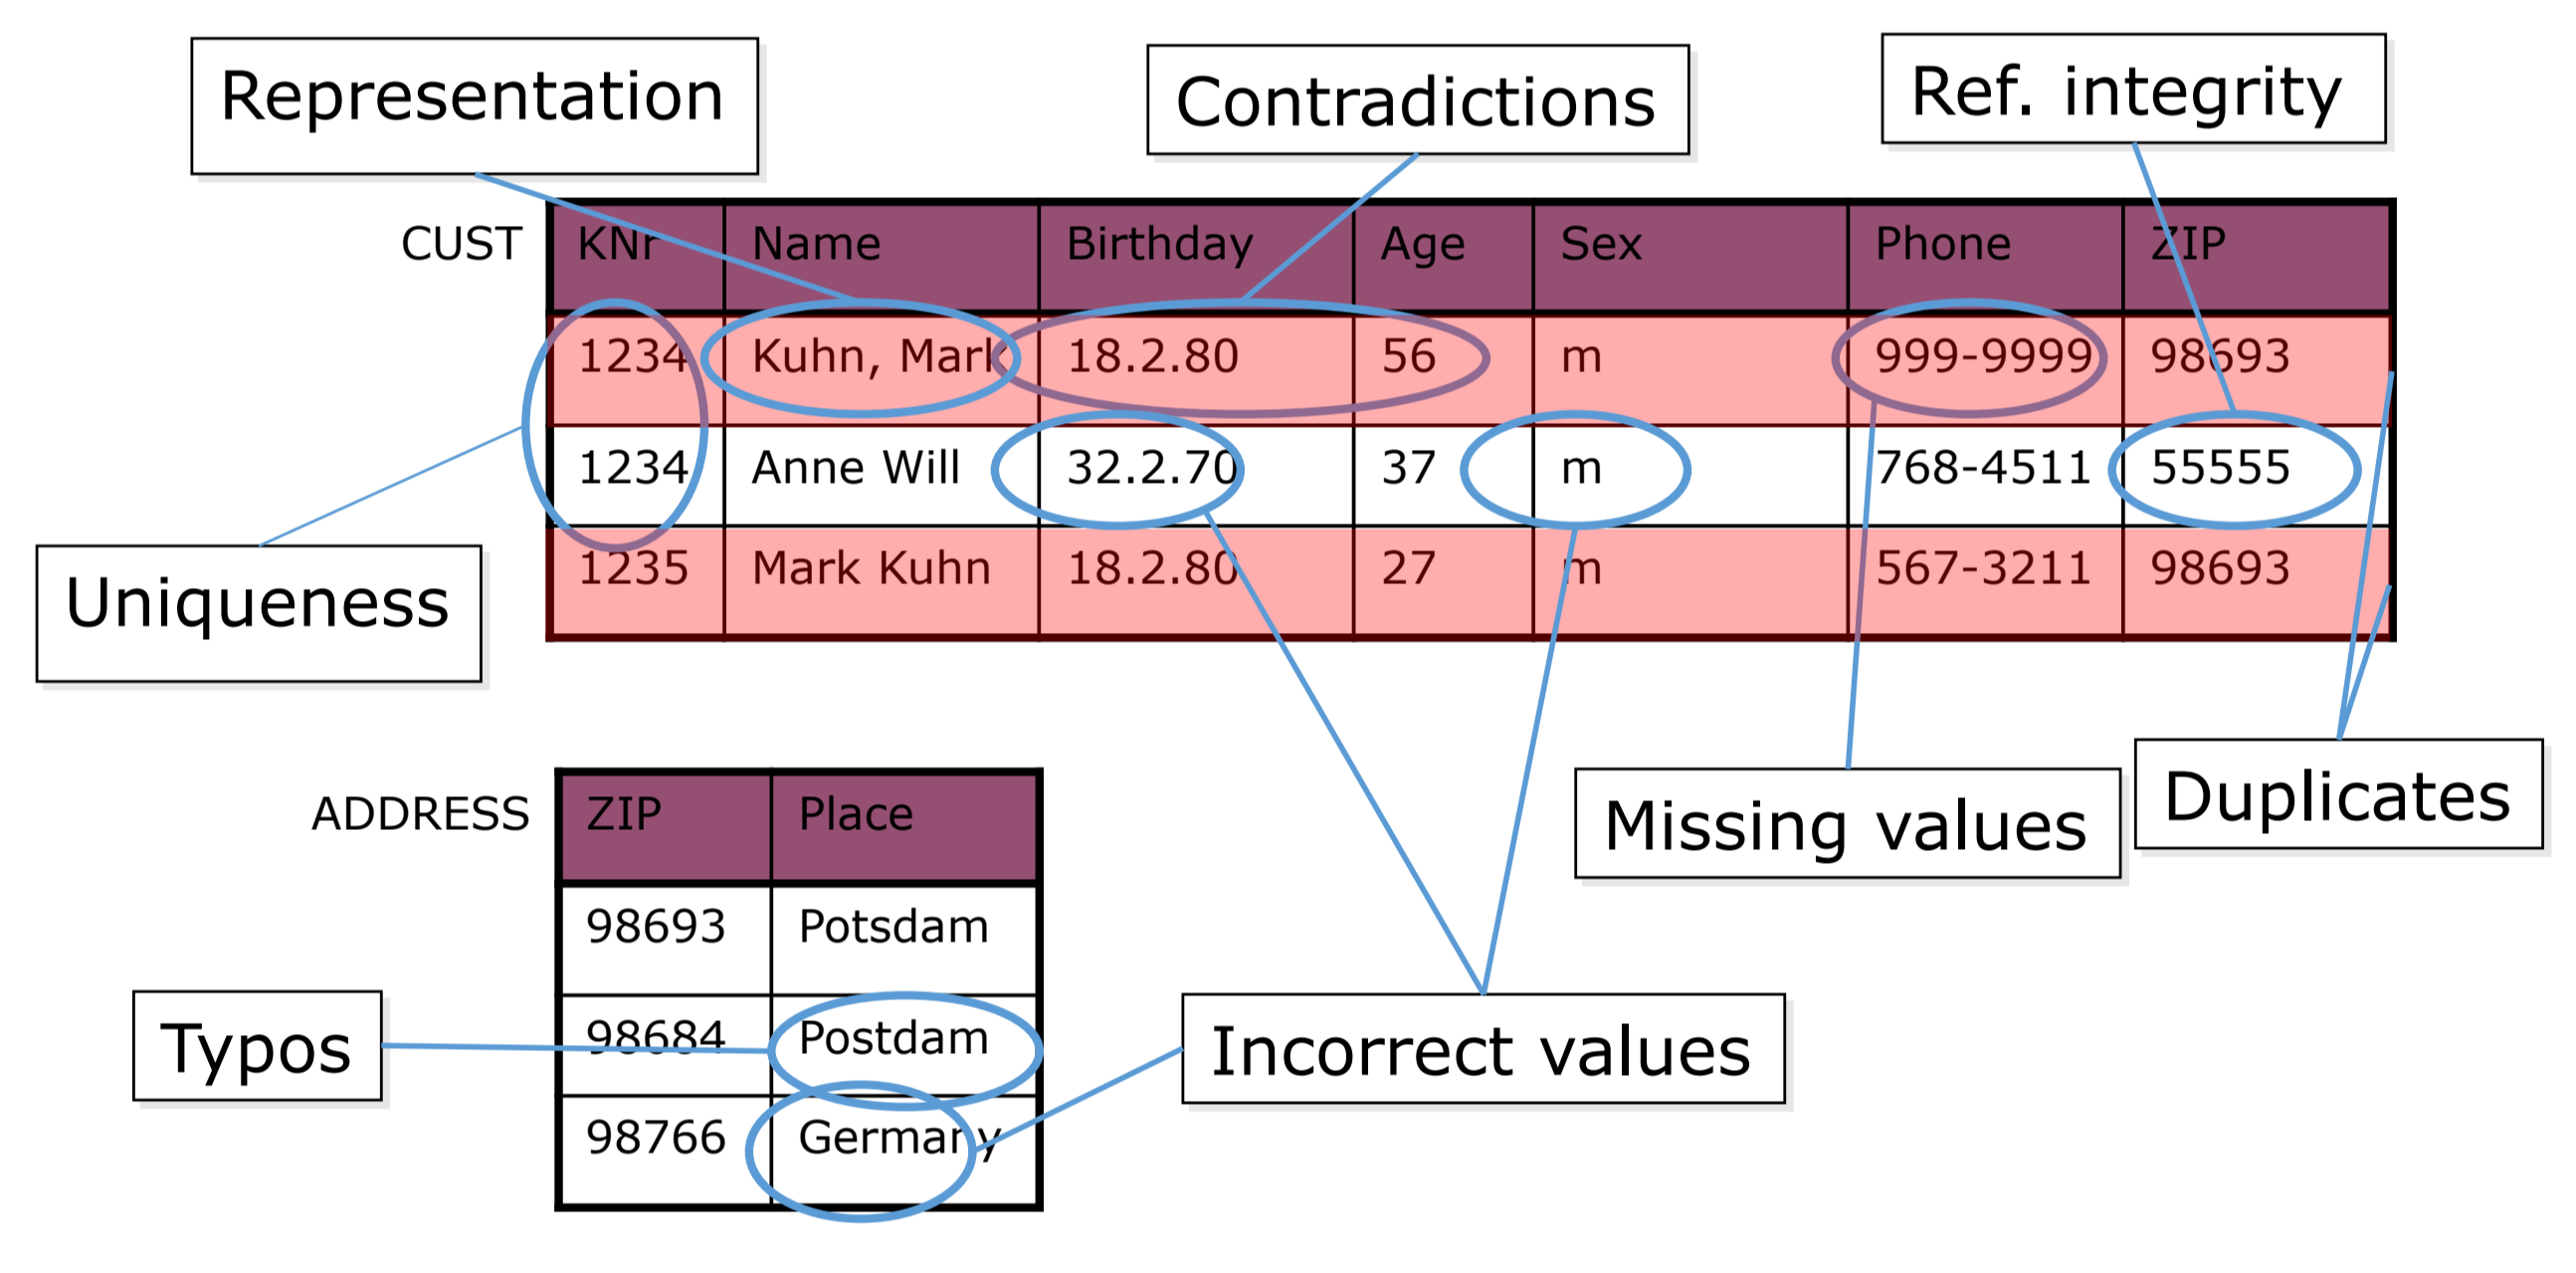
\includegraphics[width=0.8\textwidth]{bild13_dataquality_problems.png}

\end{frame}

\end{document}